\documentclass{ximera}

%\usepackage{todonotes}

\newcommand{\todo}{}

\usepackage{esint} % for \oiint
\ifxake%%https://math.meta.stackexchange.com/questions/9973/how-do-you-render-a-closed-surface-double-integral
\renewcommand{\oiint}{{\large\bigcirc}\kern-1.56em\iint}
\fi


\graphicspath{
  {./}
  {ximeraTutorial/}
  {basicPhilosophy/}
  {functionsOfSeveralVariables/}
  {normalVectors/}
  {lagrangeMultipliers/}
  {vectorFields/}
  {greensTheorem/}
  {shapeOfThingsToCome/}
  {dotProducts/}
  {partialDerivativesAndTheGradientVector/}
  {../productAndQuotientRules/exercises/}
  {../normalVectors/exercisesParametricPlots/}
  {../continuityOfFunctionsOfSeveralVariables/exercises/}
  {../partialDerivativesAndTheGradientVector/exercises/}
  {../directionalDerivativeAndChainRule/exercises/}
  {../commonCoordinates/exercisesCylindricalCoordinates/}
  {../commonCoordinates/exercisesSphericalCoordinates/}
  {../greensTheorem/exercisesCurlAndLineIntegrals/}
  {../greensTheorem/exercisesDivergenceAndLineIntegrals/}
  {../shapeOfThingsToCome/exercisesDivergenceTheorem/}
  {../greensTheorem/}
  {../shapeOfThingsToCome/}
  {../separableDifferentialEquations/exercises/}
  {vectorFields/}
}

\newcommand{\mooculus}{\textsf{\textbf{MOOC}\textnormal{\textsf{ULUS}}}}

\usepackage{tkz-euclide}
\usepackage{tikz}
\usepackage{tikz-cd}
\usetikzlibrary{arrows}
\tikzset{>=stealth,commutative diagrams/.cd,
  arrow style=tikz,diagrams={>=stealth}} %% cool arrow head
\tikzset{shorten <>/.style={ shorten >=#1, shorten <=#1 } } %% allows shorter vectors

\usetikzlibrary{backgrounds} %% for boxes around graphs
\usetikzlibrary{shapes,positioning}  %% Clouds and stars
\usetikzlibrary{matrix} %% for matrix
\usepgfplotslibrary{polar} %% for polar plots
\usepgfplotslibrary{fillbetween} %% to shade area between curves in TikZ
%\usetkzobj{all}
\usepackage[makeroom]{cancel} %% for strike outs
%\usepackage{mathtools} %% for pretty underbrace % Breaks Ximera
%\usepackage{multicol}
\usepackage{pgffor} %% required for integral for loops



%% http://tex.stackexchange.com/questions/66490/drawing-a-tikz-arc-specifying-the-center
%% Draws beach ball
\tikzset{pics/carc/.style args={#1:#2:#3}{code={\draw[pic actions] (#1:#3) arc(#1:#2:#3);}}}



\usepackage{array}
\setlength{\extrarowheight}{+.1cm}
\newdimen\digitwidth
\settowidth\digitwidth{9}
\def\divrule#1#2{
\noalign{\moveright#1\digitwidth
\vbox{\hrule width#2\digitwidth}}}




% \newcommand{\RR}{\mathbb R}
% \newcommand{\R}{\mathbb R}
% \newcommand{\N}{\mathbb N}
% \newcommand{\Z}{\mathbb Z}

\newcommand{\sagemath}{\textsf{SageMath}}


%\renewcommand{\d}{\,d\!}
%\renewcommand{\d}{\mathop{}\!d}
%\newcommand{\dd}[2][]{\frac{\d #1}{\d #2}}
%\newcommand{\pp}[2][]{\frac{\partial #1}{\partial #2}}
% \renewcommand{\l}{\ell}
%\newcommand{\ddx}{\frac{d}{\d x}}

% \newcommand{\zeroOverZero}{\ensuremath{\boldsymbol{\tfrac{0}{0}}}}
%\newcommand{\inftyOverInfty}{\ensuremath{\boldsymbol{\tfrac{\infty}{\infty}}}}
%\newcommand{\zeroOverInfty}{\ensuremath{\boldsymbol{\tfrac{0}{\infty}}}}
%\newcommand{\zeroTimesInfty}{\ensuremath{\small\boldsymbol{0\cdot \infty}}}
%\newcommand{\inftyMinusInfty}{\ensuremath{\small\boldsymbol{\infty - \infty}}}
%\newcommand{\oneToInfty}{\ensuremath{\boldsymbol{1^\infty}}}
%\newcommand{\zeroToZero}{\ensuremath{\boldsymbol{0^0}}}
%\newcommand{\inftyToZero}{\ensuremath{\boldsymbol{\infty^0}}}



% \newcommand{\numOverZero}{\ensuremath{\boldsymbol{\tfrac{\#}{0}}}}
% \newcommand{\dfn}{\textbf}
% \newcommand{\unit}{\,\mathrm}
% \newcommand{\unit}{\mathop{}\!\mathrm}
% \newcommand{\eval}[1]{\bigg[ #1 \bigg]}
% \newcommand{\seq}[1]{\left( #1 \right)}
% \renewcommand{\epsilon}{\varepsilon}
% \renewcommand{\phi}{\varphi}


% \renewcommand{\iff}{\Leftrightarrow}

% \DeclareMathOperator{\arccot}{arccot}
% \DeclareMathOperator{\arcsec}{arcsec}
% \DeclareMathOperator{\arccsc}{arccsc}
% \DeclareMathOperator{\si}{Si}
% \DeclareMathOperator{\scal}{scal}
% \DeclareMathOperator{\sign}{sign}


%% \newcommand{\tightoverset}[2]{% for arrow vec
%%   \mathop{#2}\limits^{\vbox to -.5ex{\kern-0.75ex\hbox{$#1$}\vss}}}
% \newcommand{\arrowvec}[1]{{\overset{\rightharpoonup}{#1}}}
% \renewcommand{\vec}[1]{\arrowvec{\mathbf{#1}}}
% \renewcommand{\vec}[1]{{\overset{\boldsymbol{\rightharpoonup}}{\mathbf{#1}}}}

% \newcommand{\point}[1]{\left(#1\right)} %this allows \vector{ to be changed to \vector{ with a quick find and replace
% \newcommand{\pt}[1]{\mathbf{#1}} %this allows \vec{ to be changed to \vec{ with a quick find and replace
% \newcommand{\Lim}[2]{\lim_{\point{#1} \to \point{#2}}} %Bart, I changed this to point since I want to use it.  It runs through both of the exercise and exerciseE files in limits section, which is why it was in each document to start with.

% \DeclareMathOperator{\proj}{\mathbf{proj}}
% \newcommand{\veci}{{\boldsymbol{\hat{\imath}}}}
% \newcommand{\vecj}{{\boldsymbol{\hat{\jmath}}}}
% \newcommand{\veck}{{\boldsymbol{\hat{k}}}}
% \newcommand{\vecl}{\vec{\boldsymbol{\l}}}
% \newcommand{\uvec}[1]{\mathbf{\hat{#1}}}
% \newcommand{\utan}{\mathbf{\hat{t}}}
% \newcommand{\unormal}{\mathbf{\hat{n}}}
% \newcommand{\ubinormal}{\mathbf{\hat{b}}}

% \newcommand{\dotp}{\bullet}
% \newcommand{\cross}{\boldsymbol\times}
% \newcommand{\grad}{\boldsymbol\nabla}
% \newcommand{\divergence}{\grad\dotp}
% \newcommand{\curl}{\grad\cross}
%\DeclareMathOperator{\divergence}{divergence}
%\DeclareMathOperator{\curl}[1]{\grad\cross #1}
% \newcommand{\lto}{\mathop{\longrightarrow\,}\limits}

% \renewcommand{\bar}{\overline}

\colorlet{textColor}{black}
\colorlet{background}{white}
\colorlet{penColor}{blue!50!black} % Color of a curve in a plot
\colorlet{penColor2}{red!50!black}% Color of a curve in a plot
\colorlet{penColor3}{red!50!blue} % Color of a curve in a plot
\colorlet{penColor4}{green!50!black} % Color of a curve in a plot
\colorlet{penColor5}{orange!80!black} % Color of a curve in a plot
\colorlet{penColor6}{yellow!70!black} % Color of a curve in a plot
\colorlet{fill1}{penColor!20} % Color of fill in a plot
\colorlet{fill2}{penColor2!20} % Color of fill in a plot
\colorlet{fillp}{fill1} % Color of positive area
\colorlet{filln}{penColor2!20} % Color of negative area
\colorlet{fill3}{penColor3!20} % Fill
\colorlet{fill4}{penColor4!20} % Fill
\colorlet{fill5}{penColor5!20} % Fill
\colorlet{gridColor}{gray!50} % Color of grid in a plot

\newcommand{\surfaceColor}{violet}
\newcommand{\surfaceColorTwo}{redyellow}
\newcommand{\sliceColor}{greenyellow}




\pgfmathdeclarefunction{gauss}{2}{% gives gaussian
  \pgfmathparse{1/(#2*sqrt(2*pi))*exp(-((x-#1)^2)/(2*#2^2))}%
}


%%%%%%%%%%%%%
%% Vectors
%%%%%%%%%%%%%

%% Simple horiz vectors
\renewcommand{\vector}[1]{\left\langle #1\right\rangle}


%% %% Complex Horiz Vectors with angle brackets
%% \makeatletter
%% \renewcommand{\vector}[2][ , ]{\left\langle%
%%   \def\nextitem{\def\nextitem{#1}}%
%%   \@for \el:=#2\do{\nextitem\el}\right\rangle%
%% }
%% \makeatother

%% %% Vertical Vectors
%% \def\vector#1{\begin{bmatrix}\vecListA#1,,\end{bmatrix}}
%% \def\vecListA#1,{\if,#1,\else #1\cr \expandafter \vecListA \fi}

%%%%%%%%%%%%%
%% End of vectors
%%%%%%%%%%%%%

%\newcommand{\fullwidth}{}
%\newcommand{\normalwidth}{}



%% makes a snazzy t-chart for evaluating functions
%\newenvironment{tchart}{\rowcolors{2}{}{background!90!textColor}\array}{\endarray}

%%This is to help with formatting on future title pages.
\newenvironment{sectionOutcomes}{}{}



%% Flowchart stuff
%\tikzstyle{startstop} = [rectangle, rounded corners, minimum width=3cm, minimum height=1cm,text centered, draw=black]
%\tikzstyle{question} = [rectangle, minimum width=3cm, minimum height=1cm, text centered, draw=black]
%\tikzstyle{decision} = [trapezium, trapezium left angle=70, trapezium right angle=110, minimum width=3cm, minimum height=1cm, text centered, draw=black]
%\tikzstyle{question} = [rectangle, rounded corners, minimum width=3cm, minimum height=1cm,text centered, draw=black]
%\tikzstyle{process} = [rectangle, minimum width=3cm, minimum height=1cm, text centered, draw=black]
%\tikzstyle{decision} = [trapezium, trapezium left angle=70, trapezium right angle=110, minimum width=3cm, minimum height=1cm, text centered, draw=black]


\title{More Pieces}

\begin{document}

\begin{abstract}
piecewise linear
\end{abstract}
\maketitle







Let's extend our composition of linear functions to piecewise linear functions.  Let $T$ and $g$ be two piecewise linear functions as defined below.






\[
T(v) = 
\begin{cases}
  2v-1 & \text{ if } \,  -4 < v \leq -1 \\
  -v+3 & \text{ if } \,  1 \leq v < 7
\end{cases}
\]





Graph of $y = T(v)$.
\begin{image}
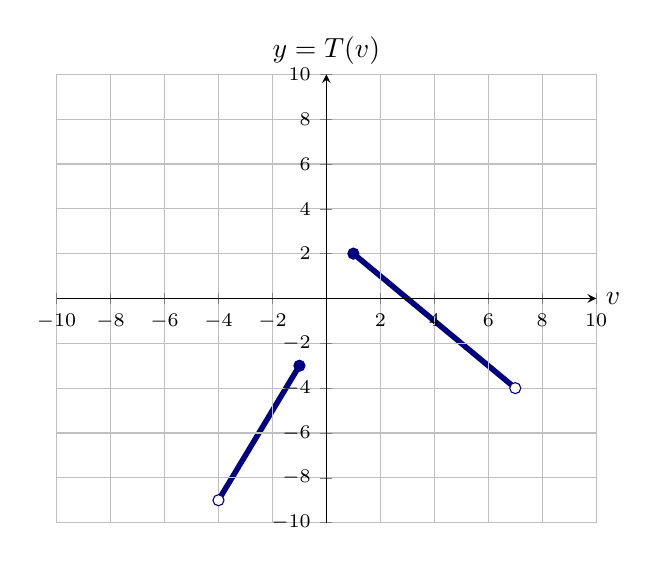
\begin{tikzpicture}
  \begin{axis}[
            domain=-10:10, ymax=10, xmax=10, ymin=-10, xmin=-10,
            axis lines =center, xlabel=$v$, ylabel={$y=T(v)$}, grid = major,
            ytick={-10,-8,-6,-4,-2,2,4,6,8,10},
            xtick={-10,-8,-6,-4,-2,2,4,6,8,10},
            ticklabel style={font=\scriptsize},
            every axis y label/.style={at=(current axis.above origin),anchor=south},
            every axis x label/.style={at=(current axis.right of origin),anchor=west},
            axis on top
          ]
          
	\addplot [draw=penColor,line width=2,smooth,domain=(-4:-1)] {2*x-1};
	\addplot [draw=penColor,line width=2,smooth,domain=(1:7)] {-x+3};
	\addplot[color=penColor,only marks,mark=*] coordinates{(-1,-3)}; 
	\addplot[color=penColor,fill=white,only marks,mark=*] coordinates{(-4,-9)}; 
	\addplot[color=penColor,only marks,mark=*] coordinates{(1,2)}; 
	\addplot[color=penColor,fill=white,only marks,mark=*] coordinates{(7,-4)}; 


    \end{axis}
\end{tikzpicture}
\end{image}





\[
g(x) = 
\begin{cases}
  -2x-3 & \text{ if }  \, -\frac{3}{2} \leq x \leq 2 \\
  \frac{7}{4}x-8 & \text{ if } \, 2 < x < 8
\end{cases}
\]

	


\begin{image}
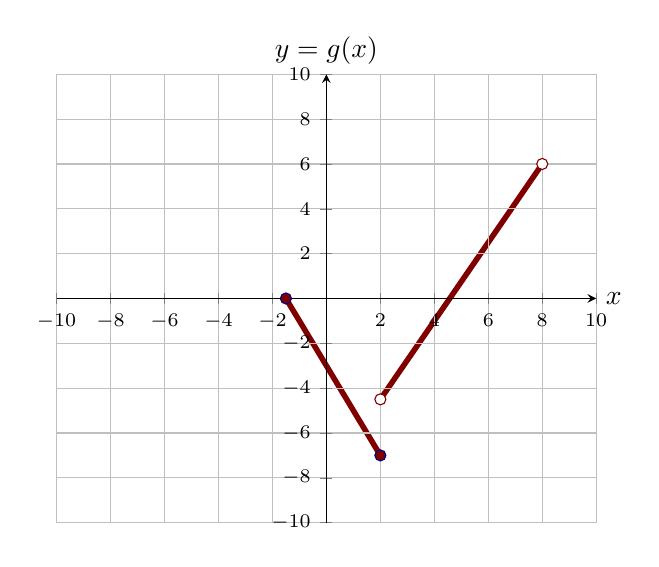
\begin{tikzpicture}
  \begin{axis}[
            domain=-10:10, ymax=10, xmax=10, ymin=-10, xmin=-10,
            axis lines =center, xlabel=$x$, ylabel={$y=g(x)$}, grid = major,
            ytick={-10,-8,-6,-4,-2,2,4,6,8,10},
          	xtick={-10,-8,-6,-4,-2,2,4,6,8,10},
          	yticklabels={$-10$,$-8$,$-6$,$-4$,$-2$,$2$,$4$,$6$,$8$,$10$}, xticklabels={$-10$,$-8$,$-6$,$-4$,$-2$,$2$,$4$,$6$,$8$,$10$},
            ticklabel style={font=\scriptsize},
            every axis y label/.style={at=(current axis.above origin),anchor=south},
            every axis x label/.style={at=(current axis.right of origin),anchor=west},
            axis on top
          ]
          
      		\addplot [line width=2, penColor2, smooth,samples=100,domain=(-1.5:2)] {-2*x-3};
          	\addplot [line width=2, penColor2, smooth,samples=100,domain=(2:8)] {1.75*x-8};




      		\addplot[color=penColor,fill=penColor2,only marks,mark=*] coordinates{(-1.5,0)};
      		\addplot[color=penColor,fill=penColor2,only marks,mark=*] coordinates{(2,-7)};


      		\addplot[color=penColor2,fill=white,only marks,mark=*] coordinates{(2,-4.5)};
      		\addplot[color=penColor2,fill=white,only marks,mark=*] coordinates{(8,6)};


           

  \end{axis}
\end{tikzpicture}
\end{image}






Let's create the composition $T \circ g = T(g)$.


This means the range of $g$ needs to be inside the domain of $T$. Since there are two pieces to each of $T$ and $g$, let's follow the pieces separately.  The chart below shows the parts of the range of $g$ coming from the individual linear pieces as well as the parts of the domain of $T$. We can see that there are numbers in the full range of $g$ that are not in the full domain of $T$.

For instance, $0$ is in the range of $g$ and not in the domain of $T$. 

We have two numbers in the domain of $g$ that $g$ maps to $0$. One from each piece.


\begin{itemize}
  \item $g\left( -\frac{3}{2} \right) = -2 \left( -\frac{3}{2} \right) - 3 = 3 - 3 = 0$
  \item $g\left( \frac{32}{7} \right) = -\frac{7}{4} \cdot \left( \frac{32}{7} \right) - 8 = 8 - 8 = 0$
\end{itemize}

We cannot include these in the domain of the composition, because they would result in $T(0)$, which is not defined.

Therefore, we cannot include $-\frac{3}{2}$ nor $\frac{32}{7}$ in the composition domain we are constructing.  

What other numbers from the domain of $g$ do we need to leave out?







\begin{image}
	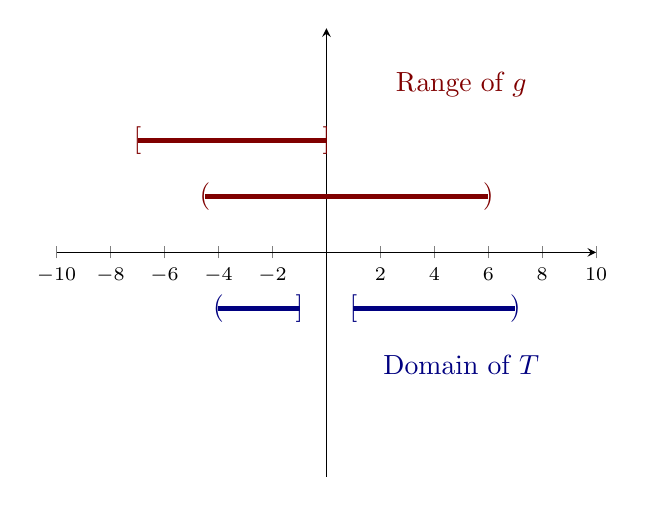
\begin{tikzpicture}
	\begin{axis}[
            domain=-10:10, ymax=2, xmax=10, ymin=-2, xmin=-10,
            %width=3in,
            clip=false,
            axis lines=center,
            %ticks=none,
            %unit vector ratio*=1 1 1,
            ymajorticks=false,
            xtick={-10,-8,-6,-4,-2,2,4,6,8,10},
            %xlabel=$x$, ylabel=$y$,
            %every axis y label/.style={at=(current axis.above origin),anchor=south},
            ticklabel style={font=\scriptsize},
            every axis x label/.style={at=(current axis.right of origin),anchor=west},
          ]      
       
          	\addplot [line width=2, penColor2, smooth,samples=100,domain=(-7:0)] ({x},{1});
          	\addplot [line width=2, penColor2, smooth,samples=100,domain=(-4.5:6)] ({x},{0.5});
          	\node at (axis cs:-7,1) [penColor2] {$[$};
          	\node at (axis cs:0,1) [penColor2] {$]$};
          	\node at (axis cs:-4.5,0.5) [penColor2] {$($};
          	\node at (axis cs:6,0.5) [penColor2] {$)$};
          	\node at (axis cs:5,1.5) [penColor2] {Range of $g$};




          	\addplot [line width=2, penColor, smooth,samples=100,domain=(-4:-1)] ({x},{-0.5});
          	\addplot [line width=2, penColor, smooth,samples=100,domain=(1:7)] ({x},{-0.5});
          	\node at (axis cs:-4,-0.5) [penColor] {$($};
          	\node at (axis cs:-1,-0.5) [penColor] {$]$};
          	\node at (axis cs:1,-0.5) [penColor] {$[$};
          	\node at (axis cs:7,-0.5) [penColor] {$)$};
          	\node at (axis cs:5,-1) [penColor] {Domain of $T$};




    \end{axis}
	\end{tikzpicture}
	\end{image}




We need to map the domain of $T$ back onto the range of $g$, find the intersection, and then work our way back into the domain of $g$, in order to restrict the domain of $g$ to just the numbers that work in the composition.


First, let's map the domain of $T$ back to the range of $g$. We need to see what each piece is doing.  So, we'll plot the domain of $T$ on the vertical axis of the graph of $g$.





\begin{image}
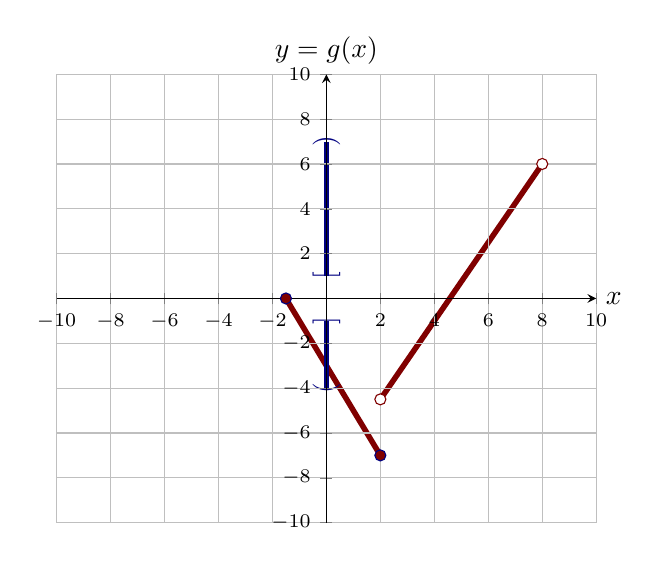
\begin{tikzpicture}
  \begin{axis}[
            domain=-10:10, ymax=10, xmax=10, ymin=-10, xmin=-10,
            axis lines =center, xlabel=$x$, ylabel={$y=g(x)$}, grid = major,
            ytick={-10,-8,-6,-4,-2,2,4,6,8,10},
          	xtick={-10,-8,-6,-4,-2,2,4,6,8,10},
          	yticklabels={$-10$,$-8$,$-6$,$-4$,$-2$,$2$,$4$,$6$,$8$,$10$}, xticklabels={$-10$,$-8$,$-6$,$-4$,$-2$,$2$,$4$,$6$,$8$,$10$},
            ticklabel style={font=\scriptsize},
            every axis y label/.style={at=(current axis.above origin),anchor=south},
            every axis x label/.style={at=(current axis.right of origin),anchor=west},
            axis on top
          ]
          
      		\addplot [line width=2, penColor2, smooth,samples=100,domain=(-1.5:2)] {-2*x-3};
          	\addplot [line width=2, penColor2, smooth,samples=100,domain=(2:8)] {1.75*x-8};
      		\addplot[color=penColor,fill=penColor2,only marks,mark=*] coordinates{(-1.5,0)};
      		\addplot[color=penColor,fill=penColor2,only marks,mark=*] coordinates{(2,-7)};
      		\addplot[color=penColor2,fill=white,only marks,mark=*] coordinates{(2,-4.5)};
      		\addplot[color=penColor2,fill=white,only marks,mark=*] coordinates{(8,6)};

      		\addplot [line width=2, penColor, smooth,samples=100,domain=(-4:-1)] ({0},{x});
      		\addplot [line width=2, penColor, smooth,samples=100,domain=(1:7)] ({0},{x});
      		\node at (axis cs:0,-4) [rotate=90, penColor] {$($};
          	\node at (axis cs:0,-1) [rotate=90, penColor] {$]$};
          	\node at (axis cs:0,1) [rotate=90, penColor] {$[$};
          	\node at (axis cs:0,7) [rotate=90, penColor] {$)$};

          	%\draw[very thick, black] (axis cs:0,0) -- (axis cs:3,5.2) node [pos=.36, above, rotate=60, black] {$\theta=\pi/3$};
           

  \end{axis}
\end{tikzpicture}
\end{image}










\begin{image}
  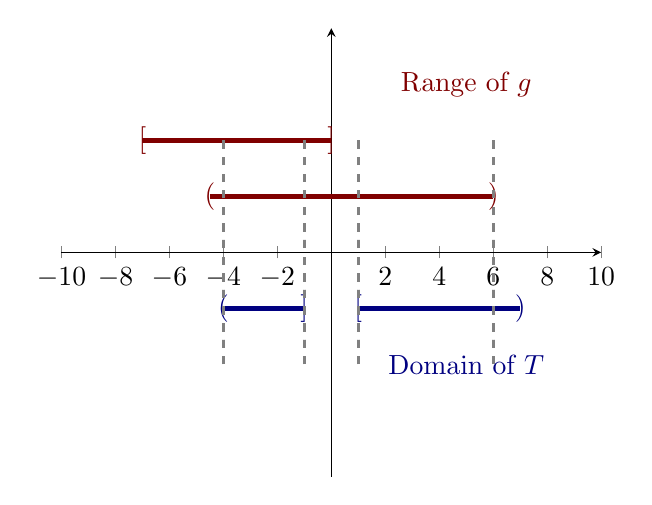
\begin{tikzpicture}
  \begin{axis}[
            domain=-10:10, ymax=2, xmax=10, ymin=-2, xmin=-10,
            %width=3in,
            clip=false,
            axis lines=center,
            %ticks=none,
            %unit vector ratio*=1 1 1,
            ymajorticks=false,
            xtick={-10,-8,-6,-4,-2,2,4,6,8,10},
            %xlabel=$x$, ylabel=$y$,
            %every axis y label/.style={at=(current axis.above origin),anchor=south},
            every axis x label/.style={at=(current axis.right of origin),anchor=west},
          ]      
       
            \addplot [line width=2, penColor2, smooth,samples=100,domain=(-7:0)] ({x},{1});
            \addplot [line width=2, penColor2, smooth,samples=100,domain=(-4.5:6)] ({x},{0.5});
            \node at (axis cs:-7,1) [penColor2] {$[$};
            \node at (axis cs:0,1) [penColor2] {$]$};
            \node at (axis cs:-4.5,0.5) [penColor2] {$($};
            \node at (axis cs:6,0.5) [penColor2] {$)$};
            \node at (axis cs:5,1.5) [penColor2] {Range of $g$};




            \addplot [line width=2, penColor, smooth,samples=100,domain=(-4:-1)] ({x},{-0.5});
            \addplot [line width=2, penColor, smooth,samples=100,domain=(1:7)] ({x},{-0.5});
            \node at (axis cs:-4,-0.5) [penColor] {$($};
            \node at (axis cs:-1,-0.5) [penColor] {$]$};
            \node at (axis cs:1,-0.5) [penColor] {$[$};
            \node at (axis cs:7,-0.5) [penColor] {$)$};
            \node at (axis cs:5,-1) [penColor] {Domain of $T$};


            \addplot [line width=1, gray, dashed,samples=100,domain=(-1:1)] ({-4},{x});
            \addplot [line width=1, gray, dashed,samples=100,domain=(-1:1)] ({-1},{x});
            \addplot [line width=1, gray, dashed,samples=100,domain=(-1:1)] ({1},{x});
            \addplot [line width=1, gray, dashed,samples=100,domain=(-1:1)] ({6},{x});





    \end{axis}
  \end{tikzpicture}
  \end{image}


The intersection is $(-4, -1] \cup [1, 6)$.



These are the common intervals in both the domain of $T$ and range of $g$.   

Now we need to connect these up to the domain of $g$.  Which parts of the domain of $g$ does $g$ map to these intervals?

Let's follow the endpoints backwards through $g$ to the domain of $g$.




Focusing on the interval endpoints (included or excluded) of this intersection, we need the preimages of $-4$, $-1$, $1$, and $6$ in the domain of $g$.  \\


$g$ has two pieces. 









$\blacktriangleright$ The interval $(-4, -1]$ is in both pieces of the range of $g$.  It has a preimage from each piece. \\


Let's examine each piece separately.  First, $-2x - 3$. \\


\begin{itemize}
\item What is the preimage of $-4$? 
\item What is the preimage of $-1$? 
\end{itemize}



Graphically, we begin at $-4$ on the vertical axis.  It is the lowest endpoint.  We follow it to the right to the graph of $g$.  Once we hit the graph, we move up until we hit the horizontal axis.  Graphically, it appears to be around $0.5$.


Graphically, we begin at $-1$ on the vertical axis.  It is the top endpoint of the lower interval.  We follow it to the left to the graph of $g$.  Once we hit the graph, we move up until we hit the horizontal axis.  Graphically, it appears to be around $-1$.






\begin{image}
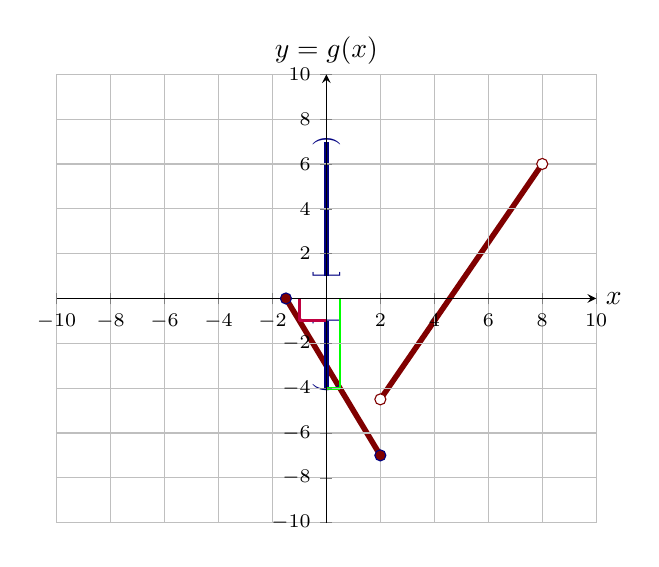
\begin{tikzpicture}
  \begin{axis}[
            domain=-10:10, ymax=10, xmax=10, ymin=-10, xmin=-10,
            axis lines =center, xlabel=$x$, ylabel={$y=g(x)$}, grid = major,
            ytick={-10,-8,-6,-4,-2,2,4,6,8,10},
            xtick={-10,-8,-6,-4,-2,2,4,6,8,10},
            yticklabels={$-10$,$-8$,$-6$,$-4$,$-2$,$2$,$4$,$6$,$8$,$10$}, xticklabels={$-10$,$-8$,$-6$,$-4$,$-2$,$2$,$4$,$6$,$8$,$10$},
            ticklabel style={font=\scriptsize},
            every axis y label/.style={at=(current axis.above origin),anchor=south},
            every axis x label/.style={at=(current axis.right of origin),anchor=west},
            axis on top
          ]
          
          \addplot [line width=2, penColor2, smooth,samples=100,domain=(-1.5:2)] {-2*x-3};
            \addplot [line width=2, penColor2, smooth,samples=100,domain=(2:8)] {1.75*x-8};
          \addplot[color=penColor,fill=penColor2,only marks,mark=*] coordinates{(-1.5,0)};
          \addplot[color=penColor,fill=penColor2,only marks,mark=*] coordinates{(2,-7)};
          \addplot[color=penColor2,fill=white,only marks,mark=*] coordinates{(2,-4.5)};
          \addplot[color=penColor2,fill=white,only marks,mark=*] coordinates{(8,6)};

          \addplot [line width=2, penColor, smooth,samples=100,domain=(-4:-1)] ({0},{x});
          \addplot [line width=2, penColor, smooth,samples=100,domain=(1:7)] ({0},{x});
          \node at (axis cs:0,-4) [rotate=90, penColor] {$($};
            \node at (axis cs:0,-1) [rotate=90, penColor] {$]$};
            \node at (axis cs:0,1) [rotate=90, penColor] {$[$};
            \node at (axis cs:0,7) [rotate=90, penColor] {$)$};

           \addplot [line width=1, purple, smooth,samples=10,domain=(-1:0)] ({x},{-1});
           \addplot [line width=1, purple, smooth,samples=50,domain=(-1:0)] ({-1},{x});


           \addplot [line width=1, green, smooth,samples=10,domain=(0:0.5)] ({x},{-4});
           \addplot [line width=1, green, smooth,samples=50,domain=(-4:0)] ({0.5},{x});


            %\draw[very thick, black] (axis cs:0,0) -- (axis cs:3,5.2) node [pos=.36, above, rotate=60, black] {$\theta=\pi/3$};
           

  \end{axis}
\end{tikzpicture}
\end{image}


Let's see if our graphical approximations are close to the actual values.



\begin{itemize}
\item $g(x) = -2x-3 = -4$
\begin{itemize}
\item $-2x = -1$
\item $x = \frac{1}{2}$
\end{itemize}
\end{itemize}

\begin{itemize}
\item $g(x) = -2x-3 = -1$
\begin{itemize}
\item $-2x = 2$
\item $x = -1$
\end{itemize}
\end{itemize}



We guessed fairly well from the graph.  We now have the preimage of the bottom interval through one piece of the formula for $g$.  


We get the interval $\left[ -1, \frac{1}{2} \right)$.


\textbf{Now for the other piece of $g$.}







The other piece of $g$ is $\frac{7}{4}x - 8$. \\


What is the preimage of $(-4, -1]$?


\begin{itemize}
\item What is the preimage of $-4$? 
\item What is the preimage of $-1$? 
\end{itemize}



Graphically, we begin at $-4$ on the vertical axis.  It is the lowest endpoint.  We follow it to the right to the other piece of the graph of $g$.  Once we hit the graph, we move up until we hit the horizontal axis.  Graphically, it appears to be around $2.25$.


Graphically, we begin at $-1$ on the vertical axis.  It is the top endpoint of the lower interval.  We follow it to the right to the graph of $g$.  Once we hit the graph, we move up until we hit the horizontal axis.  Graphically, it appears to be around $4$.





\begin{image}
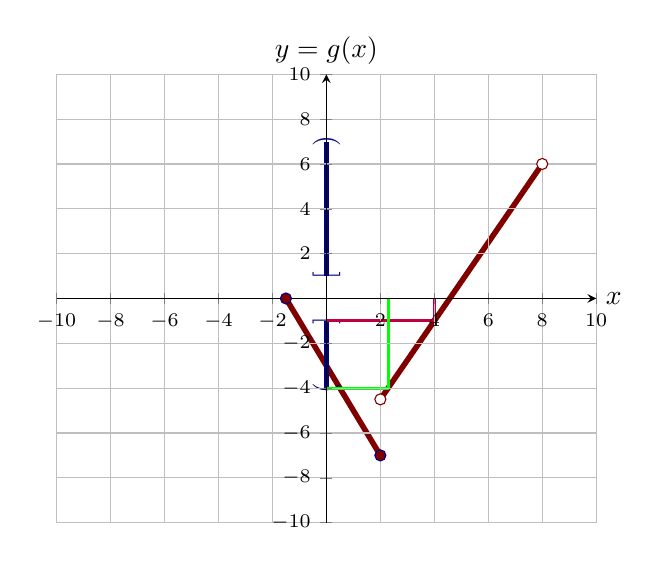
\begin{tikzpicture}
  \begin{axis}[
            domain=-10:10, ymax=10, xmax=10, ymin=-10, xmin=-10,
            axis lines =center, xlabel=$x$, ylabel={$y=g(x)$}, grid = major,
            ytick={-10,-8,-6,-4,-2,2,4,6,8,10},
            xtick={-10,-8,-6,-4,-2,2,4,6,8,10},
            yticklabels={$-10$,$-8$,$-6$,$-4$,$-2$,$2$,$4$,$6$,$8$,$10$}, xticklabels={$-10$,$-8$,$-6$,$-4$,$-2$,$2$,$4$,$6$,$8$,$10$},
            ticklabel style={font=\scriptsize},
            every axis y label/.style={at=(current axis.above origin),anchor=south},
            every axis x label/.style={at=(current axis.right of origin),anchor=west},
            axis on top
          ]
          
          \addplot [line width=2, penColor2, smooth,samples=100,domain=(-1.5:2)] {-2*x-3};
            \addplot [line width=2, penColor2, smooth,samples=100,domain=(2:8)] {1.75*x-8};
          \addplot[color=penColor,fill=penColor2,only marks,mark=*] coordinates{(-1.5,0)};
          \addplot[color=penColor,fill=penColor2,only marks,mark=*] coordinates{(2,-7)};
          \addplot[color=penColor2,fill=white,only marks,mark=*] coordinates{(2,-4.5)};
          \addplot[color=penColor2,fill=white,only marks,mark=*] coordinates{(8,6)};

          \addplot [line width=2, penColor, smooth,samples=100,domain=(-4:-1)] ({0},{x});
          \addplot [line width=2, penColor, smooth,samples=100,domain=(1:7)] ({0},{x});
          \node at (axis cs:0,-4) [rotate=90, penColor] {$($};
            \node at (axis cs:0,-1) [rotate=90, penColor] {$]$};
            \node at (axis cs:0,1) [rotate=90, penColor] {$[$};
            \node at (axis cs:0,7) [rotate=90, penColor] {$)$};

           \addplot [line width=1, purple, smooth,samples=10,domain=(0:4)] ({x},{-1});
           \addplot [line width=1, purple, smooth,samples=50,domain=(-1:0)] ({4},{x});


           \addplot [line width=1, green, smooth,samples=10,domain=(0:2.3)] ({x},{-4});
           \addplot [line width=1, green, smooth,samples=50,domain=(-4:0)] ({2.3},{x});


            %\draw[very thick, black] (axis cs:0,0) -- (axis cs:3,5.2) node [pos=.36, above, rotate=60, black] {$\theta=\pi/3$};
           

  \end{axis}
\end{tikzpicture}
\end{image}





Let's see if our graphical approximations are close to the actual values.


\begin{itemize}
\item $g(x) = \frac{7}{4}x -8 = -4$
\begin{itemize}
\item $\frac{7}{4}x = 4$
\item $x = \frac{16}{7} \approx 2.3$
\end{itemize}
\end{itemize}




\begin{itemize}
\item $g(x) = \frac{7}{4}x -8 = -1$
\begin{itemize}
\item $\frac{7}{4}x = 7$
\item $x = 4$
\end{itemize}
\end{itemize}








We guessed fairly well from the graph.  We now have the preimage of the bottom interval through the second piece of the formula for $g$.  


We get the interval $\left( \frac{16}{7}, 4 \right]$.





\textbf{Now for the other interval in the range of $g$.}




$\blacktriangleright$ The interval $[1, 6)$ has a preimage on only one piece. \\
$1$ and $6$ have preimages only through $g(x) = -2x-3$.





\begin{itemize}
\item What is the preimage of $1$? 
\item What is the preimage of $6$? 
\end{itemize}



Graphically, we begin at $1$ on the vertical axis.  It is the lower endpoint of the top interval.  We follow it to the right to the larger piece of the graph of $g$.  Once we hit the graph, we move down until we hit the horizontal axis.  Graphically, it appears to be around $5$.


Graphically, we begin at $6$ on the vertical axis.  It is the upper endpoint of the top interval of our intersection (not the top of $g$, but the top of our common interval).  We follow it to the right to the graph of $g$.  Once we hit the graph, we move down until we hit the horizontal axis.  Graphically, it appears to be around $8$.




\begin{image}
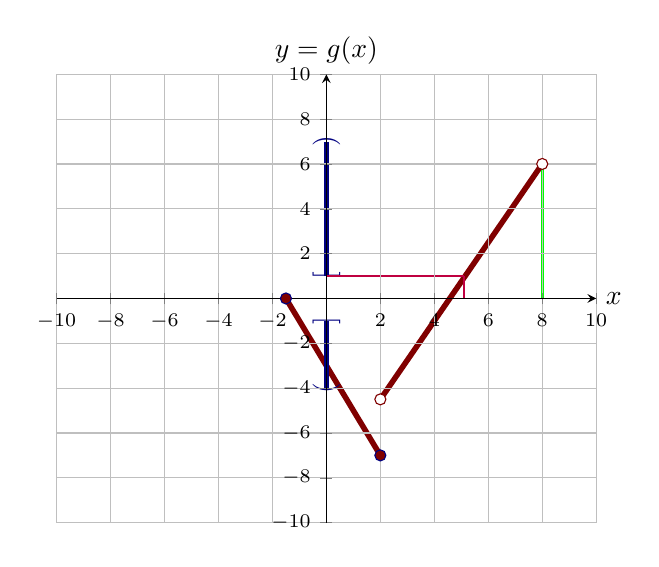
\begin{tikzpicture}
  \begin{axis}[
            domain=-10:10, ymax=10, xmax=10, ymin=-10, xmin=-10,
            axis lines =center, xlabel=$x$, ylabel={$y=g(x)$}, grid = major,
            ytick={-10,-8,-6,-4,-2,2,4,6,8,10},
            xtick={-10,-8,-6,-4,-2,2,4,6,8,10},
            yticklabels={$-10$,$-8$,$-6$,$-4$,$-2$,$2$,$4$,$6$,$8$,$10$}, xticklabels={$-10$,$-8$,$-6$,$-4$,$-2$,$2$,$4$,$6$,$8$,$10$},
            ticklabel style={font=\scriptsize},
            every axis y label/.style={at=(current axis.above origin),anchor=south},
            every axis x label/.style={at=(current axis.right of origin),anchor=west},
            axis on top
          ]
          
          \addplot [line width=2, penColor2, smooth,samples=100,domain=(-1.5:2)] {-2*x-3};
            \addplot [line width=2, penColor2, smooth,samples=100,domain=(2:8)] {1.75*x-8};
          \addplot[color=penColor,fill=penColor2,only marks,mark=*] coordinates{(-1.5,0)};
          \addplot[color=penColor,fill=penColor2,only marks,mark=*] coordinates{(2,-7)};
          \addplot[color=penColor2,fill=white,only marks,mark=*] coordinates{(2,-4.5)};
          \addplot[color=penColor2,fill=white,only marks,mark=*] coordinates{(8,6)};

          \addplot [line width=2, penColor, smooth,samples=100,domain=(-4:-1)] ({0},{x});
          \addplot [line width=2, penColor, smooth,samples=100,domain=(1:7)] ({0},{x});
          \node at (axis cs:0,-4) [rotate=90, penColor] {$($};
            \node at (axis cs:0,-1) [rotate=90, penColor] {$]$};
            \node at (axis cs:0,1) [rotate=90, penColor] {$[$};
            \node at (axis cs:0,7) [rotate=90, penColor] {$)$};

           \addplot [line width=1, purple, smooth,samples=10,domain=(0:5.1)] ({x},{1});
           \addplot [line width=1, purple, smooth,samples=50,domain=(1:0)] ({5.1},{x});


           \addplot [line width=1, green, smooth,samples=10,domain=(0:8)] ({x},{6});
           \addplot [line width=1, green, smooth,samples=50,domain=(0:6)] ({8},{x});


            %\draw[very thick, black] (axis cs:0,0) -- (axis cs:3,5.2) node [pos=.36, above, rotate=60, black] {$\theta=\pi/3$};
           

  \end{axis}
\end{tikzpicture}
\end{image}


Let's see if our graphical approximations are close to the actual values.

\begin{itemize}
\item $g(x) = \frac{7}{4}x -8 = 1$
\begin{itemize}
\item $\frac{7}{4}x = 9$
\item $x = \frac{36}{7} \approx 5.1$
\end{itemize}
\end{itemize}

\begin{itemize}
\item $g(x) = \frac{7}{4}x -8 = 6$
\begin{itemize}
\item $\frac{7}{4}x = 14$
\item $x = 8$
\end{itemize}
\end{itemize}








We guessed fairly well from the graph.  We now have the preimage of the top interval through the larger piece of $g$.  


We get the interval $\left[ \frac{36}{7}, 8 \right)$.






The domain of $T \circ g$ is $\left( -1, \frac{1}{2} \right] \cup \left( \frac{16}{7}, 4 \right] \cup \left[ \frac{36}{7}, 8 \right)$ \\


This is inside the full domain of $g$. It is not the full domain of $g$.  We needed to leave some domain numbers out, because the full domain of $g$ would give the full range of $g$, which was bigger than the domain of $T$.



There are three pieces to the domain of our composition: 


\begin{itemize}
  \item $\left[ -1, \frac{1}{2} \right)$
  \item $\left( \frac{16}{7}, 4 \right]$
  \item $\left[ \frac{36}{7}, 8 \right)$
\end{itemize}



The composition will have a formula for each piece.





\begin{explanation}



\textbf{\textcolor{purple!85!blue}{Now for the formulas}} \\


We have a composition: $T \circ g$.  We know this is a piecewise linear function, because it is the composition of two piecewise linear functions. \\

Our composition has a piecewise defined formula, let's use $c$ for its variable. \\





$\blacktriangleright$ On $\left[ -1, \frac{1}{2} \right)$




\begin{itemize}

\item the formula for $g(x)$ is $\answer{-2x-3}$
\item the image of $g(x)$ on $\left[ -1, \frac{1}{2} \right)$ is $\left( \answer{-4}, \answer{-1} \right]$
\item On $( -4, -1 ]$, the formula for $T(v) = \answer{2v-1}$  \\
\item $(T \circ g)(c) = 2 \left(\answer{-2c-3}\right) - 1 = -4c - 7$ \\


\end{itemize}








$\blacktriangleright$ On $\left( \frac{16}{7}, \answer{4} \right]$



\begin{itemize}

\item the formula for $g(x)$ is $\answer{\frac{7}{4}x - 8}$
\item the image of $g(x)$ on $\left( \frac{16}{7}, 4 \right]$ is $\left( \answer{-4}, \answer{-1} \right]$
\item On $( -4, -1 ]$, the formula for $T(v) = \answer{2v-1}$  \\
\item $(T \circ g)(c) = 2\left(\answer{\frac{7}{4}c - 8}\right) - 1 = \frac{7}{2}c - 17$ \\


\end{itemize}












$\blacktriangleright$ On $\left[ \frac{36}{7}, \answer{8} \right)$



\begin{itemize}

\item the formula for $g(x)$ is $\answer{\frac{7}{4}x - 8}$
\item the image of $g(x)$ on $\left[ \frac{36}{7}, 8 \right)$ is $\left[ \answer{1}, \answer{6} \right)$
\item On $[ 1, 6 )$, the formula for $T(v) = \answer{-v + 3}$  \\
\item $(T \circ g)(c) = -\left(\answer{\frac{7}{4}c - 8}\right) + 3 = -\frac{7}{4}c + 11$ \\


\end{itemize}

































\[
T(g(c)) = 
\begin{cases}
  -4c - 7                &       \text{ on }     \left[-1, \frac{1}{2}\right) \\
  \frac{7}{2}c - 17     &     \text{ on }  \left(\frac{16}{7}, 4\right] \\
  -\frac{7}{4}c + 11   &     \text{ on }  \left[\frac{36}{7}, 8\right)
\end{cases}
\]


  

\end{explanation}





















\begin{center}
\textbf{\textcolor{green!50!black}{ooooo-=-=-=-ooOoo-=-=-=-ooooo}} \\

more examples can be found by following this link\\ \link[More Examples of Piecewise Composition]{https://ximera.osu.edu/csccmathematics/precalculus1/precalculus1/compositionPiecewise/examples/exampleList}

\end{center}






\end{document}
